%% Beispiel-Präsentation mit LaTeX Beamer im KIT-Design
%% entsprechend den Gestaltungsrichtlinien vom 1. August 2020
%%
%% Siehe https://sdqweb.ipd.kit.edu/wiki/Dokumentvorlagen

%% Beispiel-Präsentation
\documentclass[en]{sdqbeamer} 
 
%% Titelbild
\titleimage{banner_2020_kit}

%% Gruppenlogo
\grouplogo{teco_logo.png} 

%% Gruppenname und Breite (Standard: 50 mm)
\groupname{
Chair of Pervasive Computing Systems/TECO\\
Institute of Telematics, Department of Informatics\\
}
%\groupnamewidth{50mm}

% Beginn der Präsentation

\title[Ear-Based Temperature Probing]{Ear-Based Temperature Probing: \\ Sensor Placement and Fusion for Wearable Applications}
\subtitle{Chair of Pervasive Computing Systems / TECO} 
\author[David Laubenstein]{David Laubenstein}

\date[05/10/2023]{May 10, 2023}

% Literatur 
 
\usepackage[citestyle=authoryear,bibstyle=numeric,hyperref,backend=biber]{biblatex}
\usepackage[inkscapeformat=png]{svg}
\addbibresource{presentation.bib}
\bibhang1em

\begin{document}
 
%Titelseite
\KITtitleframe

%Inhaltsverzeichnis
% sollte weg laut betreuern
% \begin{frame}{Inhaltsverzeichnis}
% \tableofcontents
% \end{frame}

\section{Motivation}
\begin{frame}{Motivation}
    \begin{itemize}
        \item Current state of temperature measurement
    \end{itemize}
    % \begin{center}
        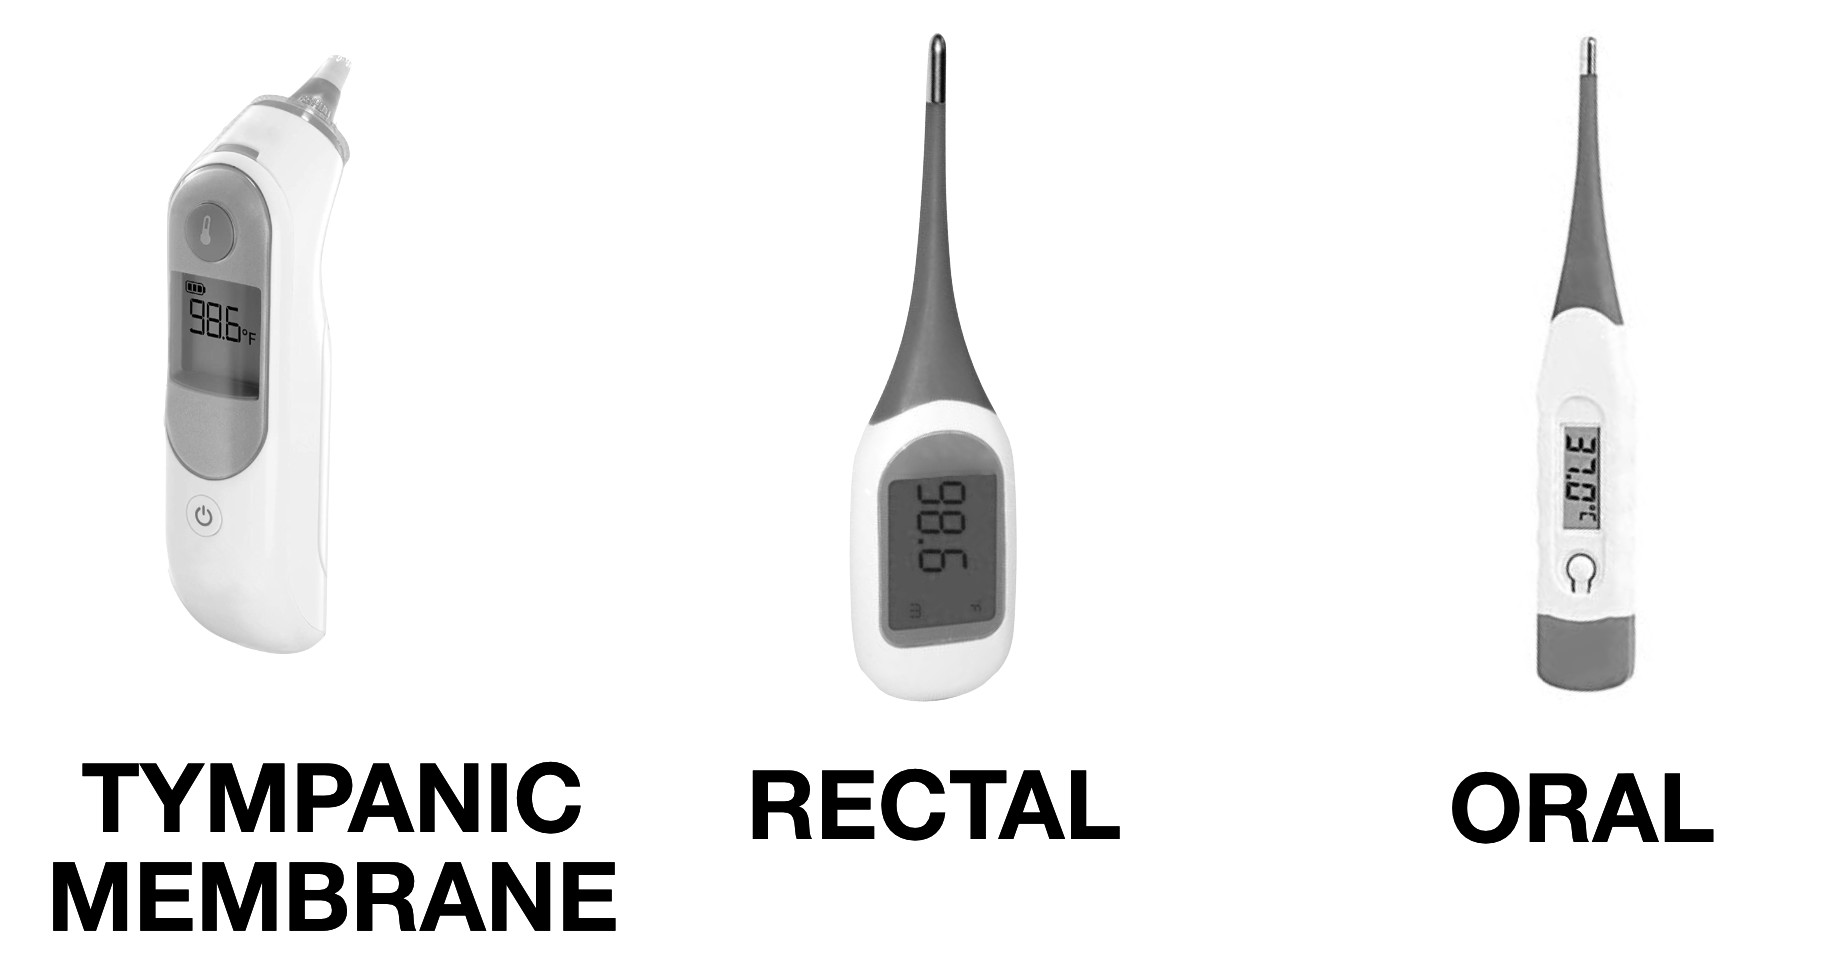
\includegraphics[scale=0.17]{proposal-presentation/images/thermometer_types.jpg}    
    % \end{center}
\end{frame}

\begin{frame}{Motivation}
    % \begin{center}
        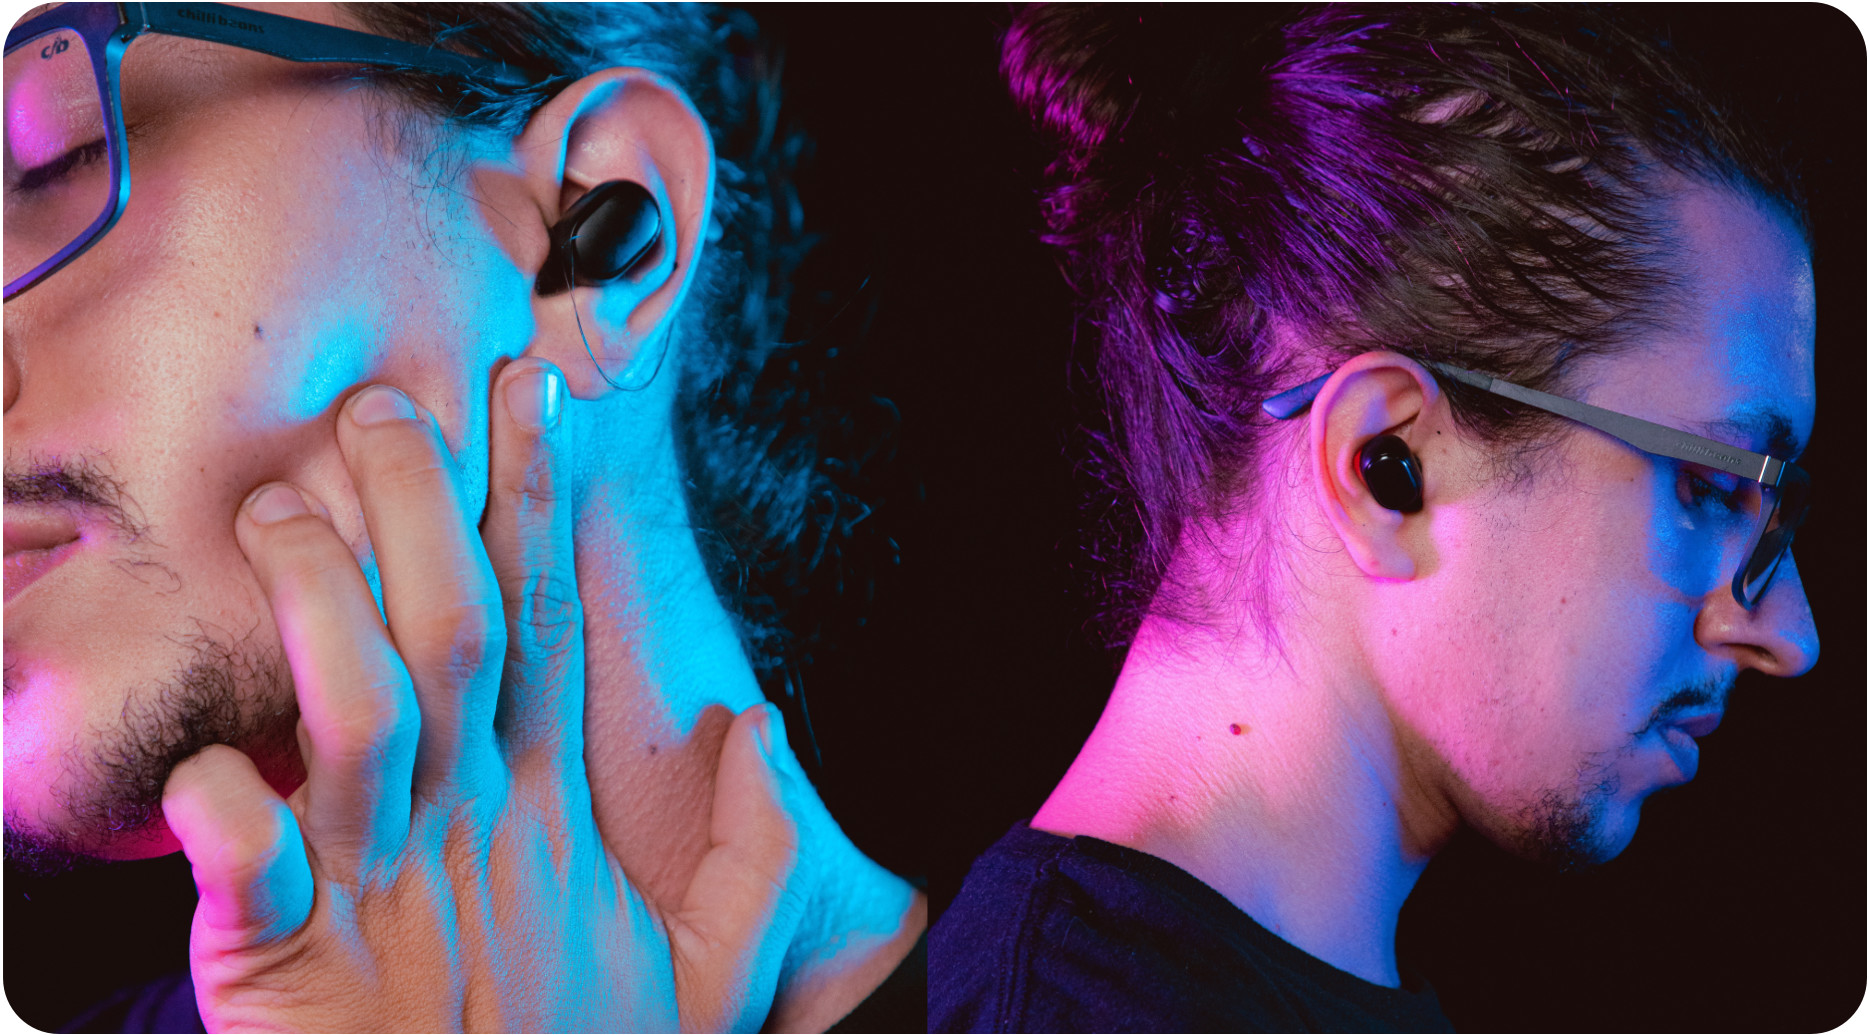
\includegraphics[scale=0.16]{proposal-presentation/images/inears/earbuds_picture.jpg}
    % \end{center}
\end{frame}

\section{Problem}
\begin{frame}{Problem}
    \begin{itemize}
        \item accuracy and reliability
        \begin{itemize}
            \item sensor location
            \item skin contact
            \item calibration
        \end{itemize}
        \item tympanic membrane measurement set up
        \begin{itemize}
            \item alignment
            \item ear wax
        \end{itemize}
    \end{itemize}
\end{frame}

\section{Question}
\begin{frame}[fragile]{Question}
    \begin{column}{0.38\textwidth}
        \begin{itemize}
            \item measure temperature at different locations in and around the ear
            \item combine resulting data to a single temperature value
            \item on different acitivties inside outside
        \end{itemize}
    \end{column}
    \begin{column}{0.58\textwidth}    
        \includegraphics[scale=0.03]{proposal-presentation/images/inears/guilherme-2.jpg}
    \end{column}
\end{frame}

\section{Planned Approach}
\begin{frame}{Planned Approach: Phase 1}
    \begin{itemize}
        \item device to measure ear-based temperature data
        \begin{itemize}
            \item OpenEarable platform adaption
            \item MLX temperature sensor
        \end{itemize}
        \item study to detect best temperature result
    \end{itemize}
    \begin{center}
        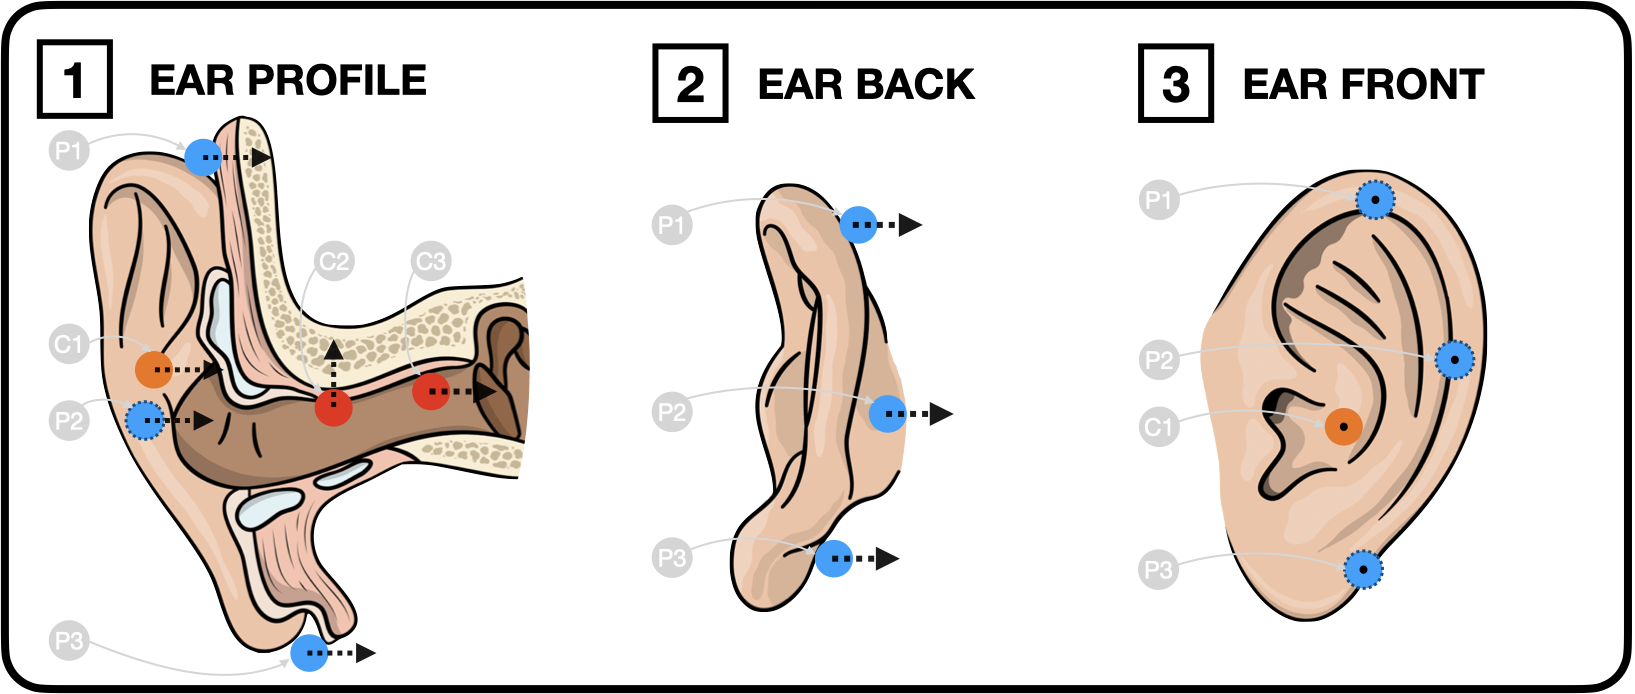
\includegraphics[scale=0.17]{../thesis-doc/images/ear_measurement_points/emp.png}    
    \end{center}
\end{frame}

\begin{frame}{Planned Approach: Phase 2}
    \begin{itemize}
        \item classify temperature-related events of the body
        \item temperature measurements during different activities
    \end{itemize}
    \begin{center}
        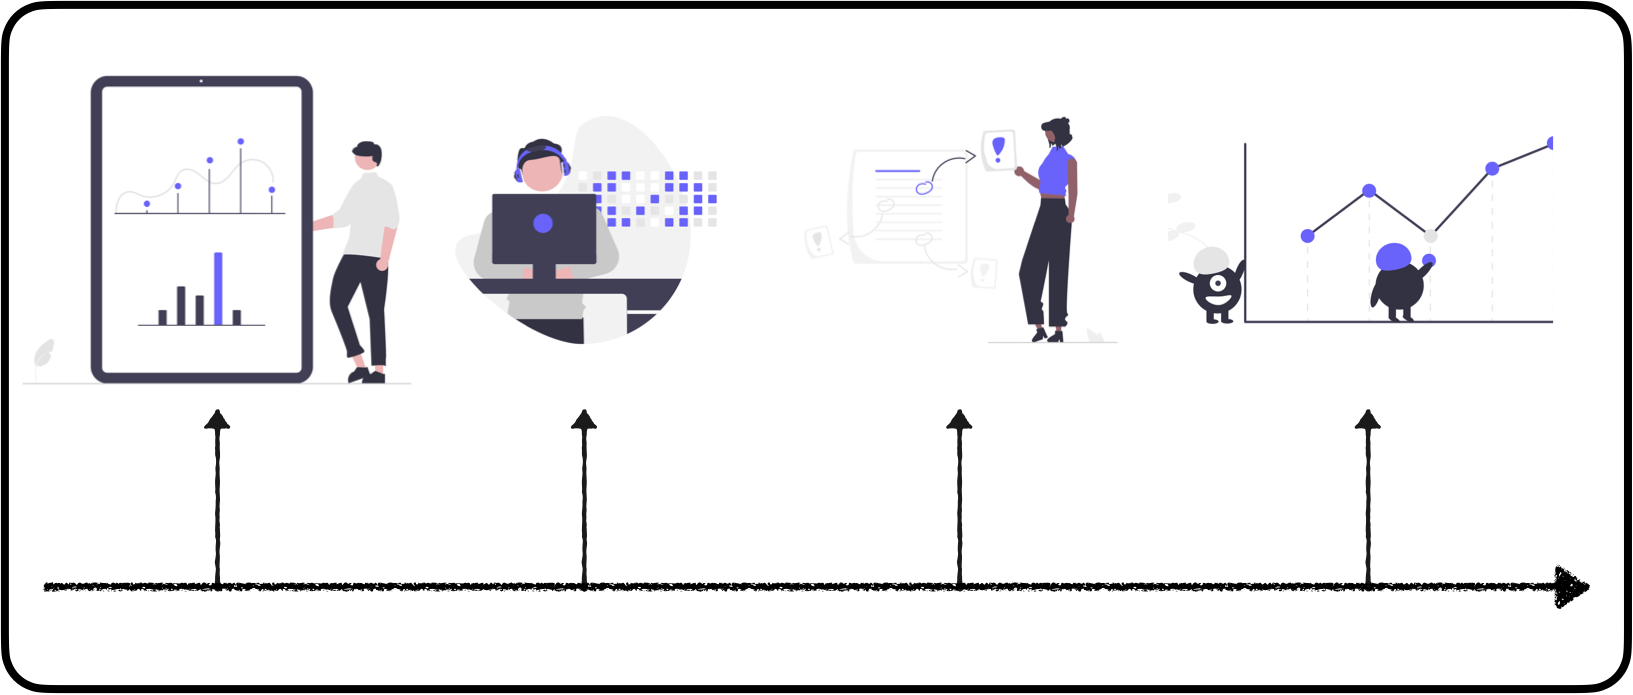
\includegraphics[scale=0.17]{proposal-presentation/images/analytics.png}    
    \end{center}
\end{frame}

\section{Expected Result}
\begin{frame}{Expected Result}
    \begin{itemize}
        \item insights into the placement of sensors for temperature monitoring in or directly on the ear
        \item is combination of multiple temperature sensors an improvement?
        \item Our results will support the development of more accurate and reliable wearable devices for biometric applications
    \end{itemize}
\end{frame}

\appendix
\beginbackup

% TODO: Add frames for appendix

% \begin{frame}{Literatur}
% \begin{exampleblock}{Titelbilder Quelle:}
%     asdf    
% \end{exampleblock}
% \end{frame}

% \begin{frame}{Literatur}
%     \printbibliography
% \end{frame}

\section{Farben}
\backupend

\end{document}